\documentclass{article}
\usepackage[T1]{fontenc}
\usepackage{lmodern}
\usepackage{graphicx}
\usepackage{amsmath,amssymb}
\usepackage[a4paper,margin=2cm]{geometry}
\usepackage[absolute,overlay]{textpos}
\setlength{\TPHorizModule}{1mm}
\setlength{\TPVertModule}{1mm}
\usepackage[indonesian]{babel}
\usepackage{hyperref}
\setlength{\emergencystretch}{2em}
% unit: Halaman 11

\begin{document}

% === Halaman 11 (llm) ===

\vspace{238.79mm}

\begin{center}\textcolor{red}{\textbf{Evariste Galois}}\end{center}

\vspace{60mm}

\begin{tabular}{ll}
Born & 25 October 1811 \\
& \textcolor{blue}{Bourgl-la-Reine}, \textcolor{blue}{French Empire} \\
\addlinespace[2mm]
Died & 31 May 1832 (aged 20) \\
& Paris, \textcolor{blue}{Kingdom of France} \\
\addlinespace[2mm]
Nationality & French \\
\addlinespace[2mm]
Fields & Mathematics \\
\addlinespace[2mm]
Known for & Work on the \textcolor{blue}{theory of equations} and \textcolor{blue}{Abelian integrals}
\end{tabular}

% deskripsi: Potret sketsa wajah Evariste Galois
% bbox normalisasi: [0.0600, 0.1080, 0.9400, 0.9120]
\begin{textblock*}{184.80mm}(12.60mm,32.08mm)
\noindent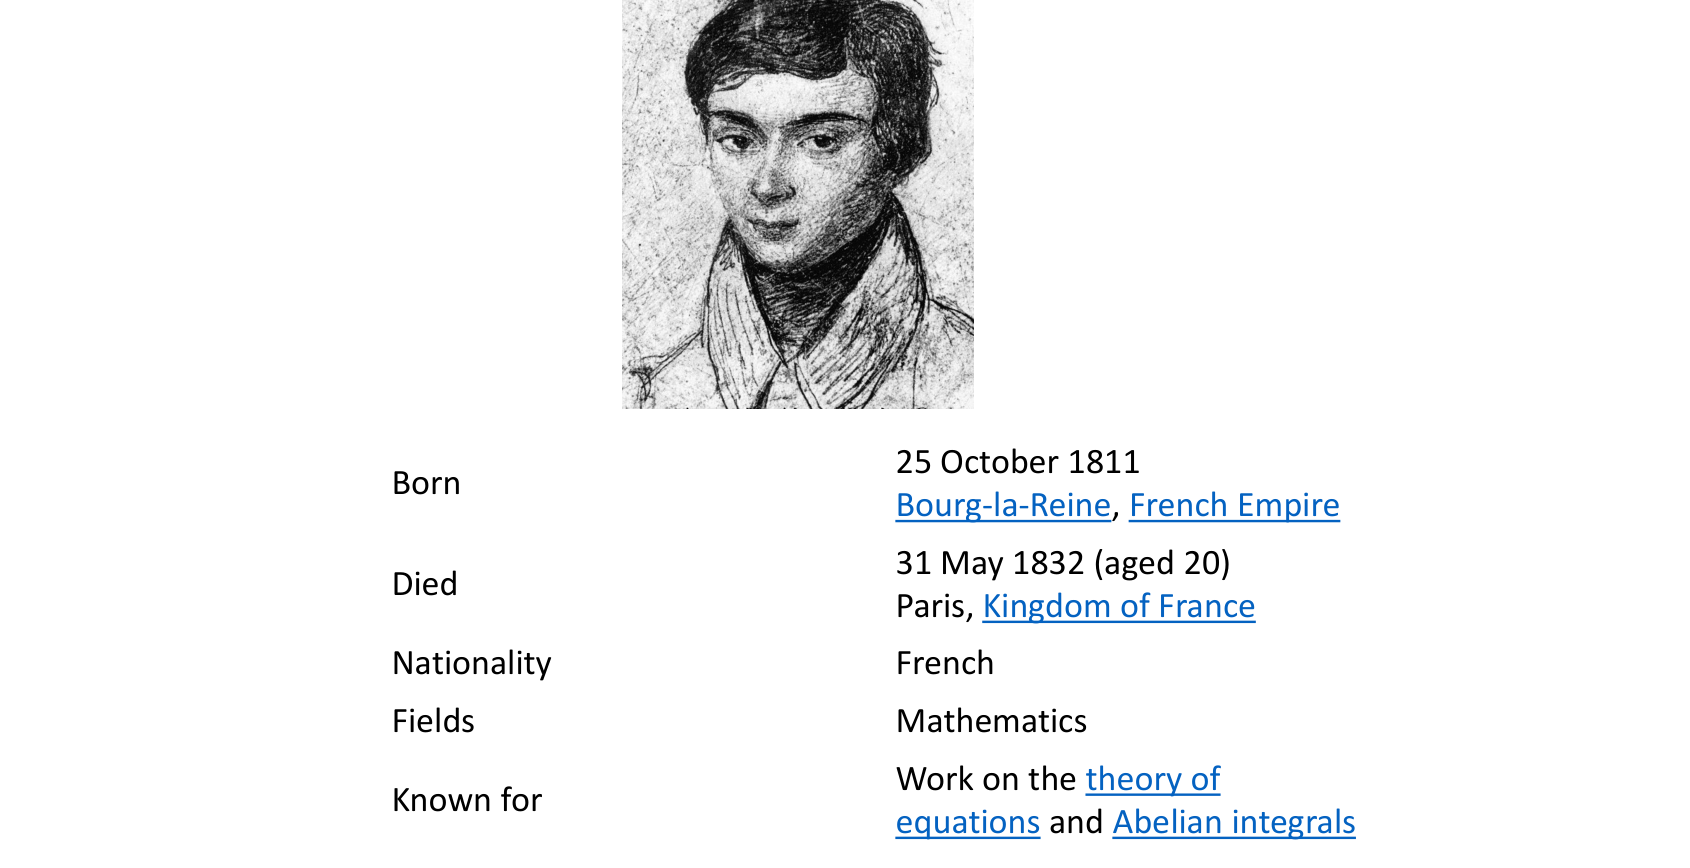
\includegraphics[width=184.80mm,height=238.79mm]{../../images/llm/page_011_img_01.png}%
\end{textblock*}

% bbox perkiraan otomatis: Potret sketsa wajah Evariste Galois

\end{document}
